We convert the circuit to its s domain equivalent and combine the inductor, capacitor and load resistance into one component denoted $Z_{eq}$:
\begin{figure}[H]
	\centering
	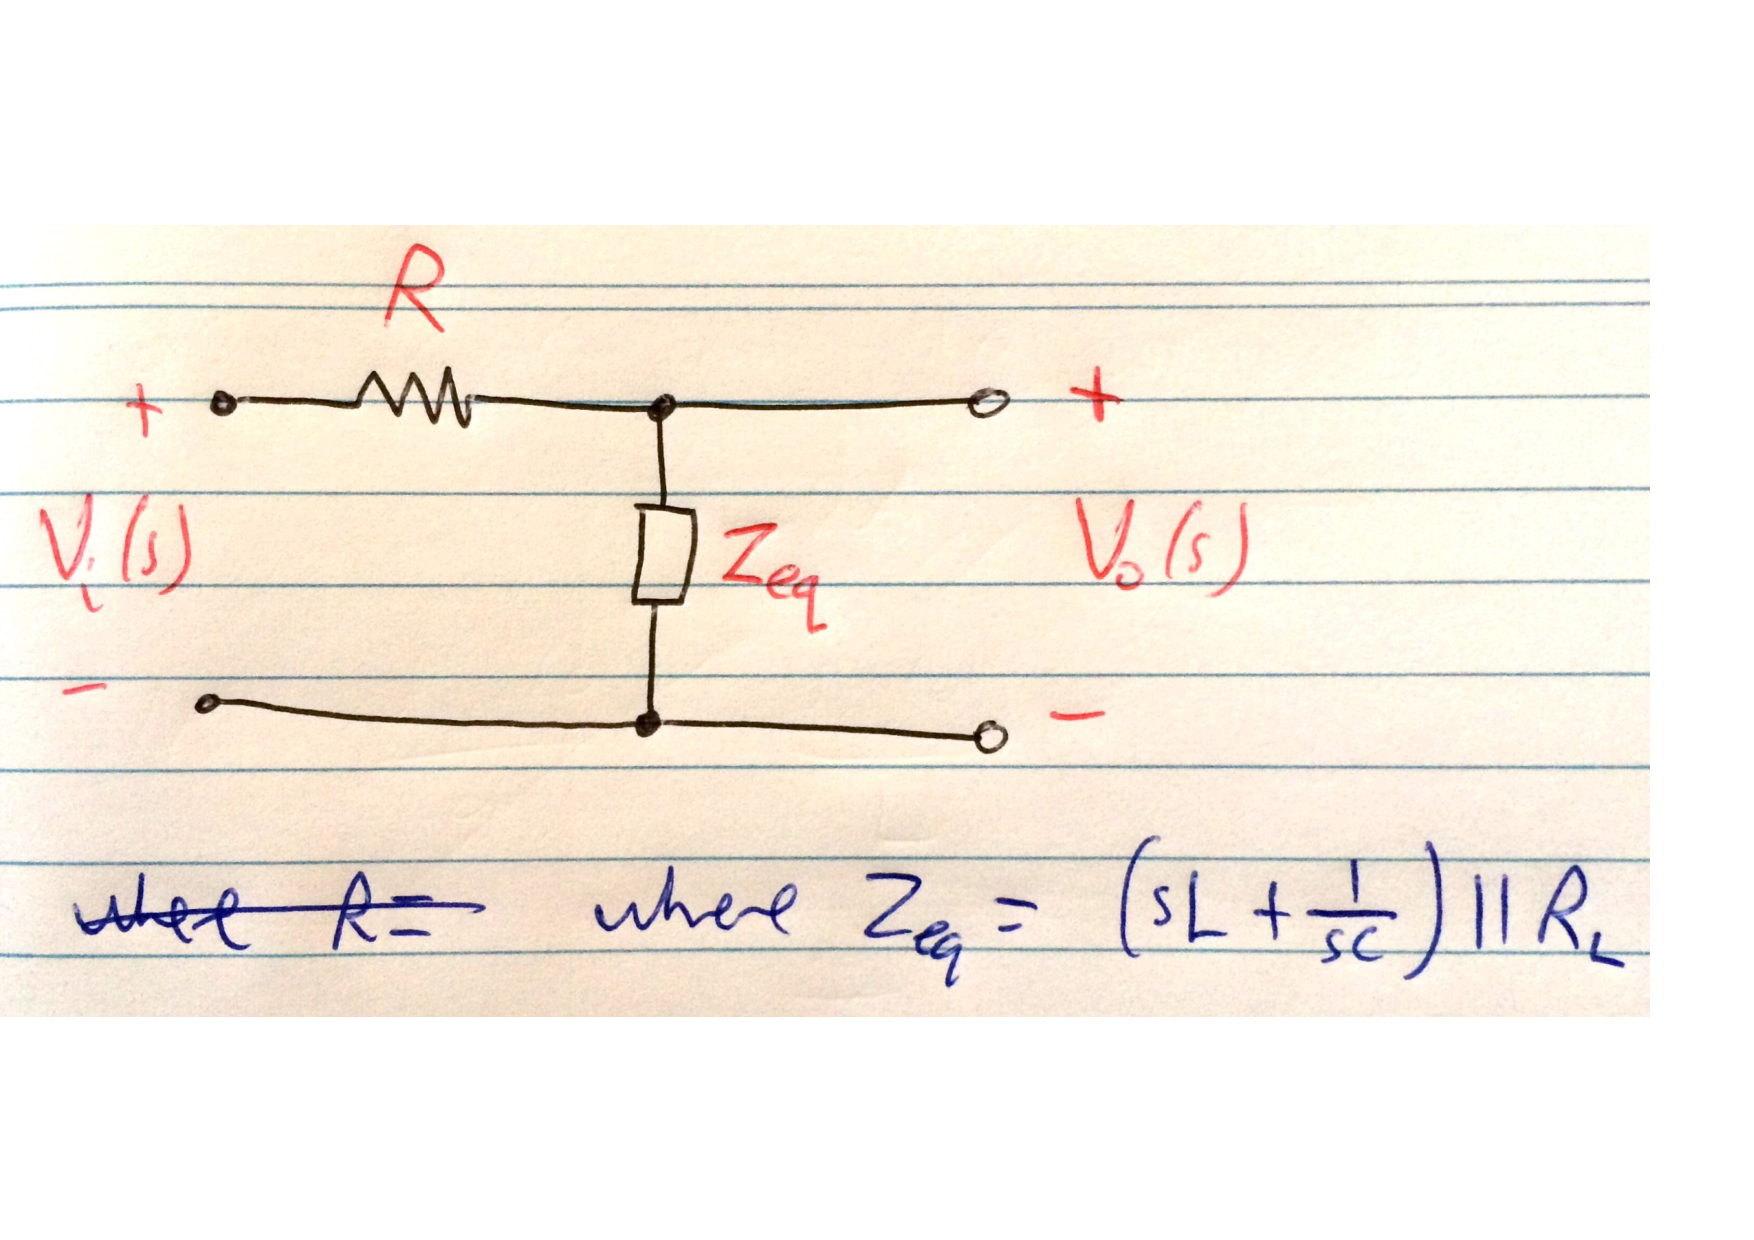
\includegraphics[scale=0.415]{q6.pdf}
\end{figure}
We note the circuit forms a voltage divider. We start by finding the impedance of the circuit across $V_o(s)$:
\begin{align*}
	Z_{eq} &= (Z_L + Z_C) \ || \ Z_R \\
	&= \left(\frac{1}{sL + \frac{1}{sC}} + \frac{1}{R_L} \right)^{-1} \\
	&= \left(\frac{sC}{s^2LC + 1} + \frac{1}{R_L} \right)^{-1} \\
	&= \left(\frac{sCR_L + s^2LC + 1}{s^2LCR_L + R_L} \right)^{-1} \\
	&= \frac{R_Ls^2 + \frac{R_L}{LC}}{s^2 + \frac{R_L}{L}s + \frac{1}{LC}} \\
	\\
	\therefore Z_{eq} &= \frac{R_L \left(s^2 + \frac{1}{LC} \right)}{s^2 + \frac{R_L}{L}s + \frac{1}{LC}}
\end{align*}
\\
Now, $V_o(s) = V_i(s)\times\frac{Z_{eq}}{R+Z_{eq}}$, and H(s) can be found from this:
\begin{align*}
	H(s) &= \frac{Z_{eq}}{R+Z_{eq}} \\
	&= \frac{R_L \left(s^2 + \frac{1}{LC} \right)}{s^2 + \frac{R_L}{L}s + \frac{1}{LC}} \times \left(\frac{R_L \left(s^2 + \frac{1}{LC} \right)}{s^2 + \frac{R_L}{L}s + \frac{1}{LC}} + R \right)^{-1} \\
	&= \frac{R_L \left(s^2 + \frac{1}{LC} \right)}{s^2 + \frac{R_L}{L}s + \frac{1}{LC}} \times \left(\frac{s^2(R_L+R) + \frac{R_LR}{L}s + \frac{1}{LC}(R_L + R)}{s^2 + \frac{R_L}{L}s + \frac{1}{LC}} \right)^{-1} \\
	&= \frac{R_L \left(s^2 + \frac{1}{LC} \right)}{s^2(R_L+R) + \frac{R_LR}{L}s + \frac{1}{LC}(R_L + R)} \\
	&= \frac{\frac{R_L}{R_L + R} \left(s^2 + \frac{1}{LC} \right)}{s^2 + \frac{R_LR}{L(R_L + R)}s + \frac{1}{LC}} \\
	\\
	\therefore H(s) &= \frac{K \left(s^2 + \frac{1}{LC} \right)}{s^2 + K \cdot \frac{R}{L}s + \frac{1}{LC}} \ , \qquad \mathrm{where} \  K = \frac{R_L}{R_L+R}
\end{align*}
